\documentclass[12pt,a4paper,latin1, frenchb]{report}
\usepackage {babel}

% Pour pouvoir utiliser 
%\usepackage{ucs}
\usepackage[T1]{fontenc}
\usepackage[latin1]{inputenc}
\usepackage {lmodern}
%\usepackage {picins} %image avec texte a ct
\usepackage{url} % Pour avoir de belles url
\usepackage {geometry}
%\usepackage{slashbox} %backslash dans tableau
%\usepackage[table]{xcolor} %couleur tableau
\usepackage{colortbl,hhline}
\usepackage{color}
\usepackage {listings} % Pour mettre du code source
\usepackage{lscape} %Pour pouvoir passer en paysage
%\usepackage {multicol} %Pour pouvoir faire plusieurs colonnes
%\usepackage{eurosym} %symbole euro
\usepackage{graphicx}
\usepackage{makeidx} %Pour crer un index
%\usepackage {setspace} %Pour l'interligne de 1.5
%\usepackage{shorttoc} %Pour crer un sommaire
\usepackage{caption}
\usepackage[font=scriptsize, format=hang]{subcaption}
%\usepackage{subfig}


\setlength{\topmargin}{-6mm}
\setlength{\textheight}{230mm}
\setlength{\textwidth}{160mm}
\setlength{\evensidemargin}{-5.45mm}
\setlength{\oddsidemargin}{-5.45mm}
 
\renewcommand{\no}{n\textsuperscript{o}}
\renewcommand{\nos}{n\textsuperscript{os}}

\renewcommand{\labelitemi}{---}
\renewcommand{\labelitemii}{$\star$}


\usepackage[pdftex, 					% Paramtrage de la navigation
bookmarks = true, 						% Signets
bookmarksnumbered = true, 				% Signets numrots
pdfpagemode = UseOutlines, 					% None, UseThumbs, UseOutlines, Fullscreen
pdfstartview = Fit, 					% FitH, FitV, FitR, FitB, FitBH, FitBV, Fit
pdfpagelayout = SinglePage, 				% SinglePage, OneColumn, TwoColumnLeft, TwoColumnRight
colorlinks = false, 					% Liens en couleur
urlcolor = black, 						% Couleur des liens externes
pdfborder = {0 0 0} 					% Style de bordure : ici, rien
]{hyperref}


\hypersetup{
    unicode=false,          % non-Latin characters in Acrobat's bookmarks
    pdftoolbar=true,        % show Acrobat's toolbar?
    pdfmenubar=true,        % show Acrobat's menu?
    pdffitwindow=true,     % window fit to page when opened
    pdftitle={Rapport de projet tuteur�},    % title
    pdfauthor={Pinto Dos Santos Almeida Catherine, Meilhac Beno�t},     % author
    pdfsubject={Transformation d'un diagramme de s�quences SysML vers les automates d'interfaces et v�rification de compatibilit� avec l'outil Ticc},   % subject of the document
    pdfcreator={Pinto Dos Santos Almeida Catherine, Meilhac Benoit},   % creator of the document
    pdfproducer={Texlive (pdflatex)}, % producer of the document
    pdfnewwindow=true,      % links in new window
}


\graphicspath{{images/}}
\newcommand{\sommaire}{\shorttoc{Sommaire}{0}}
\makeindex
\definecolor{gris}{gray}{0.75}
\definecolor{orange}{rgb}{1,0.5,0}
\definecolor{vert}{rgb}{0,0.75,0}


% Pour les marges de la page
%\geometry{a4paper, top=2.5cm, bottom=3.5cm, left=1.5cm, right=1.5cm, marginparwidth=1.2cm}
\geometry{a4paper}

% Pour les entetes de page
\usepackage{fancyhdr}


\parskip=5pt %% distance entre les (paragraphe)
\sloppy %% respecter toujours la marge de droite 

% Pour les p�nalit�s :
\interfootnotelinepenalty=150 %note de bas de page
\widowpenalty=150 %% veuves et orphelines
\clubpenalty=150 

%Pour la longueur de l'indentation des paragraphes
\setlength{\parindent}{15mm}

%%%% debut macro pour enlever le nom chapitre %%%%
\makeatletter
\def\@makechapterhead#1{%
  \vspace*{50\p@}%
  {\parindent \z@ \raggedright \normalfont
    \interlinepenalty\@M
    \ifnum \c@secnumdepth >\m@ne
        \Huge\bfseries \thechapter\quad
    \fi
    \Huge \bfseries #1\par\nobreak
    \vskip 40\p@
  }}

\def\@makeschapterhead#1{%
  \vspace*{50\p@}%
  {\parindent \z@ \raggedright
    \normalfont
    \interlinepenalty\@M
    \Huge \bfseries  #1\par\nobreak
    \vskip 40\p@
  }}
\makeatother
%%%% fin macro %%%%

%redfinition maketitle pour mettre en haut de page
\makeatletter
\renewcommand{\maketitle}{%
    \vspace*{0.5cm}% ICI La taille que tu veux avant le titre
    
    \begin{center}%
    {\large
     \lineskip .75em%
      \begin{tabular}[t]{c}%
        \@author
      \end{tabular}\par}%
    \vskip 2em%
    
    {\large \@date \par}%       % Set date in \large size.
    
      \vskip 1.5em%
    {\textbf{\LARGE \@title} \par}%
    \end{center}\par
    \vskip 1.5em%
	\thispagestyle{empty}% virer numrotation
	\setcounter{page}{0}% remettre compteur au dbut
	\clearpage
	\newpage
}
\makeatother

%Couverture 

\title{
	\normalsize{D�partement informatique\\
	Universit� de Franche-Comt�\\
	Projet tuteur�\\
	Ann�e 2011-2012}\\
	\vspace{15mm}
}

\author{Catherine PINTO DOS SANTOS ALMEIDA\\Beno�t MEILHAC  %rajouter un \\ au besoin
	\vspace{5mm}
}

\date{
	\begin{center} 
	%	
\includegraphics[width=7cm]{ufc.jpg}
        
\includegraphics[scale=0.15]{ufc.jpg}
	\end{center}
	\vspace{5mm}
	\huge{\textbf{Transformation d'un diagramme de s�quences SysML vers les automates d'interfaces et v�rification de compatibilit� avec l'outil Ticc}}\\
	\vspace{14mm}
	\normalsize{	
	Tuteurs :\\
        Mr MOUNTASSIR\\
        Mr HAMMAD\\
        Mr CHOUALI
	}
}


\begin{document}
\pagestyle{empty}
\maketitle

%\pagenumbering{Roman} 
\setcounter{page}{1} 

%\input{Abstract}

%\input{Acknowledgment}

\tableofcontents
\clearpage
\newpage

%\sommaire
%\addcontentsline{toc}{chapter}{Sommaire}
%\clearpage

%\pagenumbering{arabic} 
%\setcounter{page}{1} 

\pagestyle{fancy}
\renewcommand{\chaptermark}[1]{\markboth{#1}{}} 
\renewcommand{\sectionmark}[1]{\markright{#1}} 

\chapter{Introduction}

De mani�re g�n�rale, pour fiabiliser le fonctionnement d'un syst�me avant son implantation sur une machine, on doit l'�tudier en amont. 

Les  phases de sp�cification et de v�rification sont devenues incontournables dans le cycle de vie pour du logiciel dans l'industrie. 

C'est pour ces raisons que l'on doit parler de la v�rification de sys�mes pour augmenter le degr� de confiance dans leur fonctionnement futur. 

En ce qui concerne le projet, il est int�ressant de s'int�resser � des syt�mes bas�s sur une architecture � composants. Avant le d�ploiment sur une machine, il est important de v�rifier dans un premier temps sa coh�rence et en particulier la compatibilit� entre composants.

SysML\protect\footnote{System Modeling Language} est une extension du langage UML\protect\footnote{Unified Modeling Language} sp�cialis� dans la mod�lisation, la sp�cification et la documentation de syst�mes. 
Les am�liorations qu'il apporte par rapport � UML lui ont permis d'accro�tre sa popularit� tant dans l'industrie que dans le milieu universitaire.
SysML introduit de nouveaux concepts comme la disparition des classes UML au profit de blocs qui sont l'unit� de base de la structure d'un syst�me (logiciel ou mat�riel). Ainsi le diagramme de classes UML est remplac� par le diagramme de d�finition de blocs (BDD\protect\footnote{Block Definition Diagram}). Celui-ci met en avant la hi�rarchie du syst�me et les diff�rentes interactions entre les composants.
Ces interactions peuvent �tre repr�sent�es sous forme d'un diagramme de s�quences mod�lisant les �changes de messages dans le temps.
Cependant, la mod�lisation ne permet pas � elle seule de v�rifier et valider la compatibilit� des composants entre eux.

Dans un mod�le bas� sur les composants, la v�rification de compatibilit� entre composants est introduite par la notion d'automates d'interfaces. Ils servent � d�crire les diff�rentes interactions d'entr�es/sorties donc le comportement d'un composant avec son environnement.

C'est dans ce contexte que se situe le projet. Partant d'un diagramme de d�finition de blocs, tous les blocs ayant des interactions avec d'autres donnent acc�s � des diagrammes de s�quences associ�s. Ces diagrammes sont ensuite transform�s en automates d'interfaces. Une v�rification de leur compatibilit� est alors possible.

Dans un premier temps, une premi�re partie sera consacr�e � fixer le cadre du projet ainsi que les diff�rents outils qui ont �t� utilis�s. Ensuite, une deuxi�me partie exposera la mise en \oe{}uvre du projet. Et en dernier lieu, les diff�rents probl�mes qui ont �t� rencontr�s.

\clearpage


%\section{Pr�sentation du sujet}

\subsection{Le sujet}
\begin{frame}{Le sujet}
    \begin{block}{Probl�matique}
        \begin{itemize}
            \item Mod�lisation graphique : SysML
            \item V�rification de l'assemblage de blocs
            \item N�cessit� d'un langage formel

        \end{itemize}

    \end{block}

\end{frame}

%

\subsection{SysML}
\begin{frame}{SysML}
    \begin{block}{Qu'est-ce que SysML ?}
        \begin{itemize}
            \item Langage de mod�lisation graphique
            \item Bas� sur UML
            \item Adapt� � l'Ing�nierie Syst�me (syst�mes complexes h�t�rog�nes)

        \end{itemize}

    \end{block}

\end{frame}

\begin{frame}{Points communs et divergences}
    \centering
    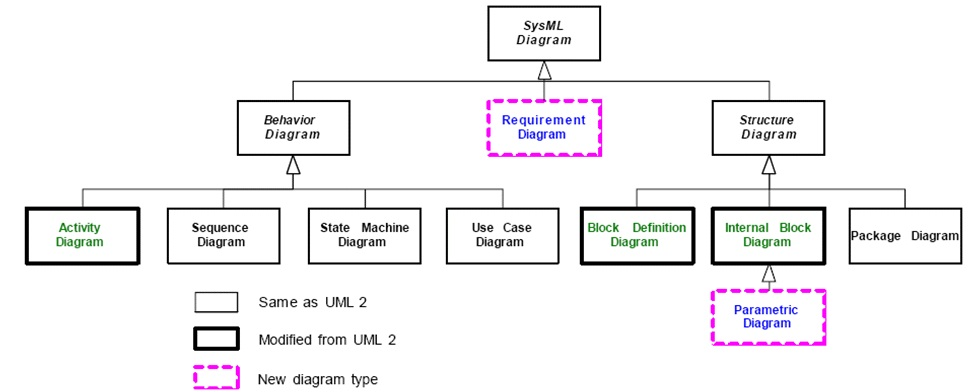
\includegraphics[scale=0.45]{./images/image5.jpg}

\end{frame}

%

\subsection{Automate d'interface}
\begin{frame}{}
    \centering
    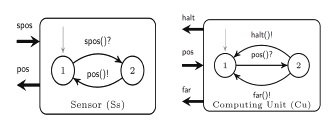
\includegraphics[scale=0.9]{./images/exempleAutomateInterface.jpg}
    \begin{block}{D�finition}
        \begin{itemize}
            \item Introduit par Alfaro et Henzinger
            \item Mod�lise les interface des composants
            \item Description des actions internes/entr�e/sortie

        \end{itemize}

    \end{block}

\end{frame}

%

\subsection{Vue globale du projet}
\begin{frame}{}
    \centering
    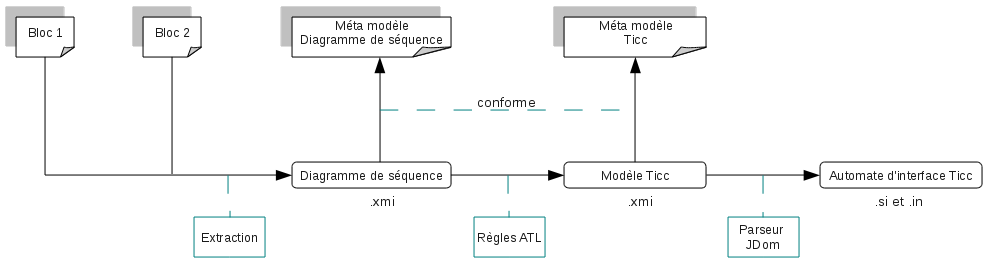
\includegraphics[scale=0.45]{./images/vueEnsemble.png}

\end{frame}





\section{R�alisation}

\subsection{Transformation de mod�les}
\begin{frame}{M�ta mod�le}
	\begin{block}{Signification}
		\begin{itemize}
			\item Grec \textit{m�ta} : changement, succession, transformation
			\item Niveau d'abstraction sup�rieur
			\item Un mod�le repr�sentant un mod�le
		
		\end{itemize}			
	
	\end{block}

\end{frame}

\begin{frame}{Transformation de mod�les}
	\centering
	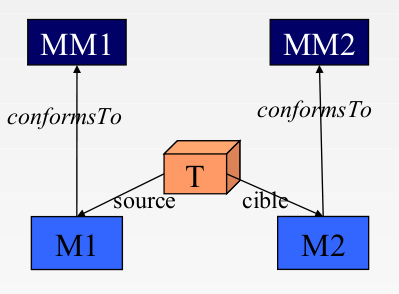
\includegraphics[scale=0.5]{./images/exogene.png}

	\begin{block}{Passage d'un mod�le � un autre}
		\begin{itemize}
			\item Mod�le source conforme � son m�ta mod�le
			\item Mod�le cible conforme � son m�ta mod�le
			\item Application de r�gles de transformation en utilisant les m�ta mod�les source et cible
		
		\end{itemize}			
	
	\end{block}

\end{frame}

%

\subsection{Les m�ta mod�les}
\begin{frame}{Diagramme de s�quences}
    \centering
    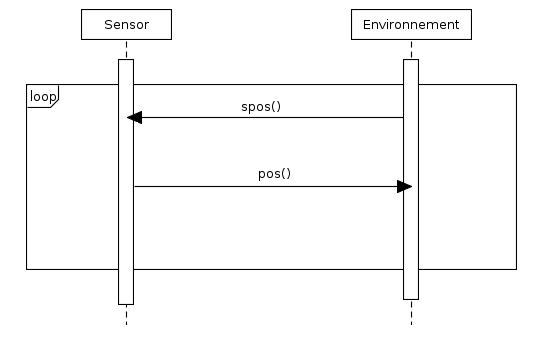
\includegraphics[scale=0.25]{./images/diagSeqExemple.png}

    \begin{block}{Simplifications}
        \begin{itemize}
            \item Red�finition de noms
            \item Abandon synchronisation des messages
            \item Garde les �l�ments utiles
            \item Ajoute de nouveaux �l�ments

        \end{itemize}

    \end{block}

\end{frame}

\begin{frame}{M�ta mod�le du diagramme de s�quences SysML}
    \centering
    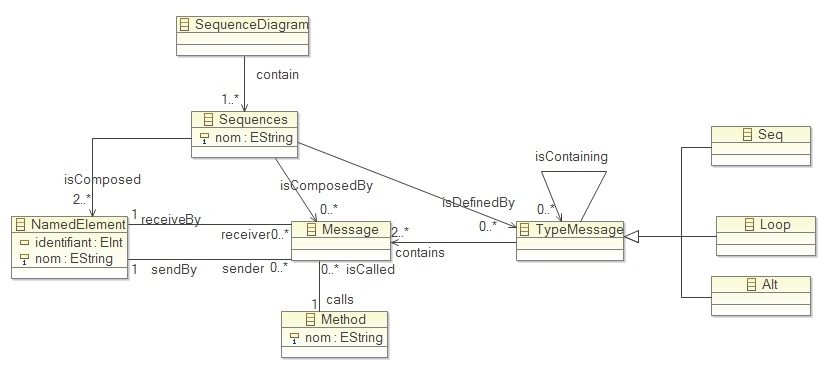
\includegraphics[scale=0.5]{./images/MMDiagSeq.jpg}

\end{frame}

\begin{frame}{M�ta mod�le du langage Ticc}
    \centering
    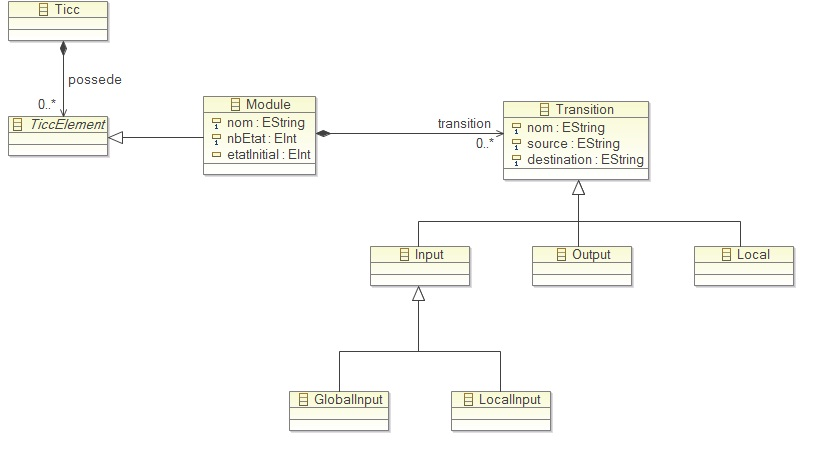
\includegraphics[scale=0.5]{./images/MMTicc.jpg}

\end{frame}

%

\subsection{Exemple fichier conforme au diagramme de s�quences}
\begin{frame}{\'Ecriture d'un fichier d'entr�e}
    \begin{block}{Explications}
        \begin{itemize}
            \item Fichier de type XMI (XML Metadata Interchange)
            \item Conforme au m�ta mod�le du diagramme de s�quences
            \item Contient deux s�quences
            \item Une s�quence re�oit/envoi des messages de/� l'ext�rieur 
            vers un composant appel� \textit{Environnement} 

        \end{itemize}

    \end{block}

\end{frame}

%

\subsection{R�gles ATL}
\begin{frame}{But des r�gles ATL}
    \centering
    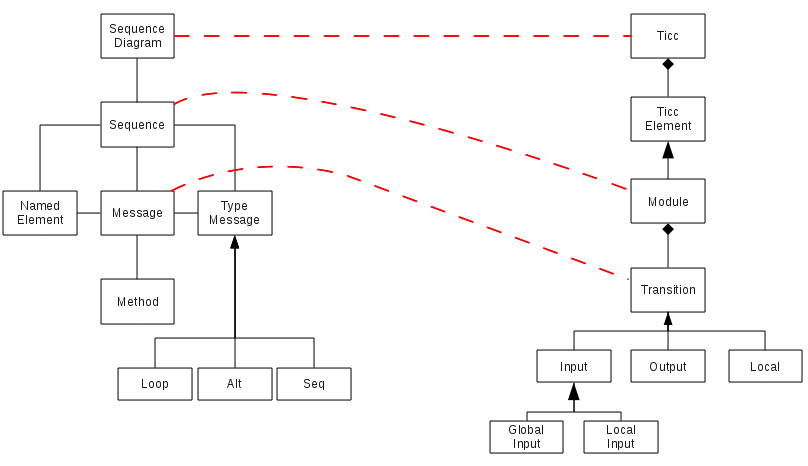
\includegraphics[scale=0.5]{./images/figureSimilitudeSeqTicc.png}

\end{frame}

%

\subsection{Parseur XML}
\begin{frame}{Parseur XML}
    \centering
    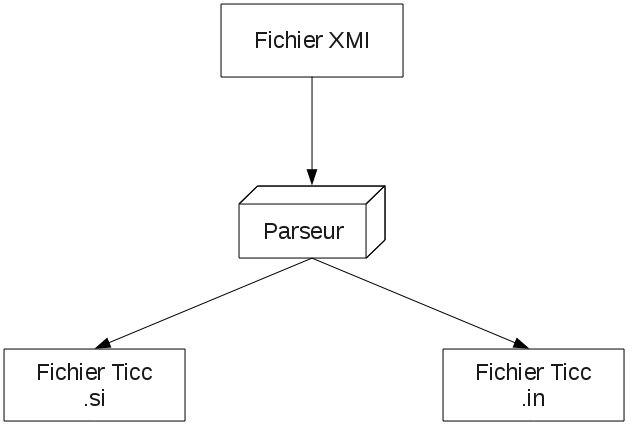
\includegraphics[scale=0.3]{./images/figureParseur.jpg}

    \begin{block}{Fonctionnement}
        \begin{itemize}
            \item Fichier de sortie XMI conforme Ticc 
            \item Traitement avec JDom
            \item G�n�ration fichier .si contenant les modules
            \item G�n�ration fichier .in ex�cutable OCaml

        \end{itemize}

    \end{block}

\end{frame}

%

\subsection{V�rification avec Ticc}
\begin{frame}{V�rification avec Ticc}
	\begin{block}{Principes}
		\begin{itemize}
			\item V�rification de compatibilit� de deux modules
			\item Utilisation des fichiers .si et .in
			\item Actuellement un fichier r�sultat trop volumineux
		
		\end{itemize}	
	
	\end{block}

\end{frame}



%\section{Bilan et Perspectives}
\begin{frame}{Bilan et perspectives}
	\begin{block}{Bilan}
		\begin{itemize}
			\item Transformation de mod�le 
			\item Ouverture � la v�rification de compatibilit�
		
		\end{itemize}
	
	\end{block}

	\begin{block}{Perspectives}
		\begin{itemize}
			\item Automatiser le processus avec un plugin Eclipse	
			\item Adapter un algorithme de parcours de BDD		
		
		\end{itemize}
	
	\end{block}

\end{frame}

\section*{}
\begin{frame}
	\centering
	\LARGE{Merci de votre attention.}

\end{frame}

\clearpage
\newpage

%\input{Glossaire}

%%----------------------------------------
%% Pour la bibliographie
%%----------------------------------------
%% Citer tous les ouvrages/rfrences
%nocite{*}
%% Trier par ordre d'apparition
%bibliographystyle{unsrt}
%% Pour le style de la biblio
%bibliographystyle{plain}
%% Ecrire la biblio ici
%bibliography{Bibliographie}
%addcontentsline{toc}{chapter}{Bibliography}

\clearpage
\newpage

\printindex

\appendix

\listoftables
\addcontentsline{toc}{chapter}{Liste des tableaux}
\clearpage

\listoffigures
\addcontentsline{toc}{chapter}{Table des figures}
\clearpage


\end{document}
